\documentclass{article}
\usepackage[utf8]{inputenc}
\usepackage{authblk}
\usepackage{graphicx}
\usepackage{hyperref}
\usepackage[numbers]{natbib}
\usepackage[export]{adjustbox}
\begin{document}

\title{Topic 1 - ImageNet Classification with Deep Convolutional Neural Networks\cite{krizhevsky2012imagenet}}
\author[1]{Ayush Mahant}
\author[2]{Alex Krizhevsky}
\author[2]{Geoffrey E. Hinton}
\affil[1]{IIITDELHI}
\affil[2]{University of Toronto}

\date{27th September 2020}
\maketitle
\begin{abstract}
 The authors have classified 1000 classes from a collection of 1.2 million high-resolution images by training a deep convolutional deep network, which was considerable. This was an initiative for the ImageNet LSVRC-2010. The authors had to train it a little faster, so they used nonsaturated neurons. An efficient GPU had to be implemented for the five convolution layers and introduced a new method called “dropout” for the three fully connected layers in the network. This was done to reduce overfitting. The authors introduced some variances in this model, thus achieving a winning error rate of 15.3 in 2012, \textbf{ImageNet LSVRC}.

  
  
 
\end{abstract}


\section{Introduction}
For better current approaches towards object recognition, collecting more massive datasets and preventing overfitting techniques is standard.   Recently, a large dataset of millions of labeled images was made possible. \textbf{Label Me}\cite{russell2008labelme} had full segmented images, and \textbf{\emph{ImageNet}}\cite{deng2009imagenet} had about 25 million high-resolution images but had a problem of complex object recognition. CNN(Convolutional neural network) has prior knowledge of datasets and controls the nature of images. THE current GPU, have advanced 2D connections and can train large CNN's well along with ImageNet. As stated by the authors, the paper's contributions are- largest CNN was used on ImageNet in \textbf{ILSVRC-2010} and 2012 competitions\cite{berg2010large}. The new neural network contains more features for improved performance and reduced training time. There still was a problem of overfitting because of the network size.

\section{Dataset}
ImageNet has 15 million labeled high-resolution images, marked using Amazon's Mechanical Turk crowdsourcing tools. The authors have said that they performed most on ILSVRC 2010. Top 5 error rate is a fraction of test images among the five labels considered the correct model is not a part of. The authors' working system requires constant input dimensionality and a fixed 256 x 256 resolution. Thus specific changes like rescaling had to be done. 

\section{Architecture} 

\subsection{ReLU Nonlinearity}
For input ‘x’ and output ‘f’ the model of neutrons  is $f(x)=tanh(x)$ or
$f(x)=(1+e^{-x})^{-1}$.
Saturation nonlinearities are slower than no saturation nonlinearities $f(x)=max(0,x)$.
The authors say that they  refer to this nonlinearity as rectified linear units\textbf{(ReLU)}
Figure Fig.\ref{fig:my_label3} shows iterations to reach 25\% training error on CIFAR -10 dataset.
\begin{figure}[h]
 \centering
    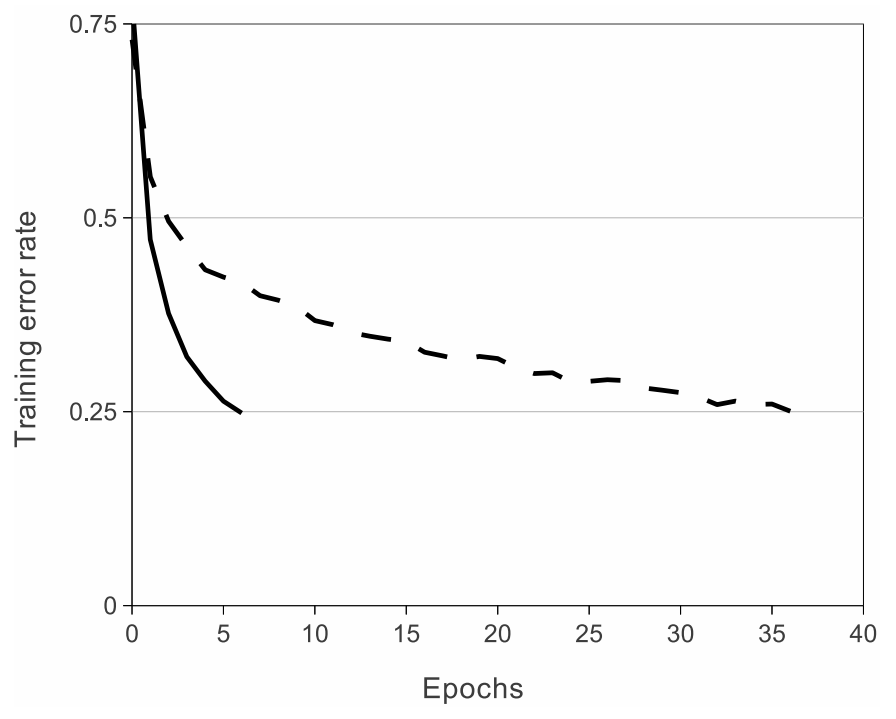
\includegraphics[width=.5\textwidth,right]{pic.png}
    \caption{25\% training error on CIFAR}
    \label{fig:my_label3}
\end{figure}
\subsection{Training on multiple GNU}
\textbf{GTX 580} GPUs have 3GB of memory, thus restraining the training due to network size. Today GPUs can read and write in one other’s memory directly and are suited for GPU parallelization. Also, the authors employed a scheme of communication of GPUs only in certain layers.  Level 3 kernels take input from kernel maps in layer 2.
\subsection{Local Response Normalization}
According to the authors, following normalization helps in generalizing the model. It is given by \newline
$b^{i}_{x,y}= {a^{i}_{x,y}}/{(k+\alpha{\sum_{j=max(0,i-n/2)}^{min(N-1,i+n/2)}{(a_{x,y}^j)^2)}}^\beta}$
\vspace{0.2in}


Where $\beta^{i}_{x.y}$ is the response normalized activity, N is total kernels
K,n, alpha and beta are hyper parameters.This model is usually termed as \textbf{“brightness normalization”}\cite{jarrett2009best}.
\subsection{Overlapping pooling}
The neighbouring group of neurons have size z x z, and the pooling layer can be considered as a grid of s spaced pixel.When s$<$ z overlapping pooling occurs. For s=2,z=3 it reduces the errors. 


\subsection{Overall architecture}
In  Fig. \ref{fig:my_label4} is shown the overall architecture of the CNN.The kernels of second, fourth and fifth convolutional layers are connected to the previous layers. Max pooling follows the layers for response normalization. 
The first convolution layer filters 224x224x3 input images whose output is input to the second one and this carries on.
\begin{figure}[h]
 \centering
    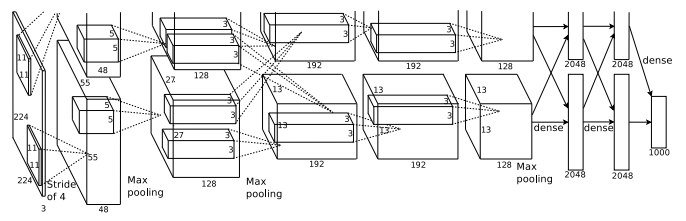
\includegraphics[width=.8\textwidth]{pic2.png}
    \caption{25\% training error on CIFAR}
    \label{fig:my_label4}
\end{figure}

\section{Reducing overfitting}
There are two ways to reduce overfitting-
\subsection{Data augmentation}
The schemes the authors used were computationally free as the transformed images in their implementation were in Python on CPU. During testing time 5 224x 224 patches are averaged to them by the network's production.The other alters into RGB channels intensities  to each RGB image pixel.
\subsection{Dropout}
The other technique is \textbf{“Dropout”}\cite{hinton2012improving} where every hidden neuron is set to zero with half a probability and reduces adaptation of neurons which is complex.

\section{Details of learning}
To reduce model’s training error the weight decay was used with updated rule for w was-
$$v_{i+1} := 0.9 .v_i -0.0005 . \epsilon . w_i - \epsilon . {\langle
{\frac{\partial L}{\partial w}{w_i}}\rangle}_{D_i}$$

$$ w_{i+1} := w_i + v_{i+1}$$
\vspace{0.1in}
Here i is the iterative index,
v is momemtum, epsilon is learning rate ${D_i}$ is the derivative wrt to w.
The weights in each layer were initialized along with biases where equal learning rate was adjusted.
\section{Result}
The authors’ results on ILSVR-2010 are in Table 1 with error rate- 37.5\% for top1 and 17.0 for top5. For ILSVR 2012, Table 2. Displays the results. The author details that error  rates of the 2012 competition are not public.

\begin{table}[!htb]
\centering
\begin{tabular}{|l|r|c|}
\hline
\textbf{{Model}} & \textbf{{Top -1}}& \textbf{{Top-5}} \\ \hline
\emph{Sparse coding\cite{berg2010large}} & \emph{47.1\%} & \emph{28.2\%} \\ \hline
\emph{SIFT + FVs\cite{sanchez2011high}} & \emph{45.7\%} & \emph{25.7\%} \\ \hline
{CNN} & {37.5\%} & {17.0\%} \\ \hline
    \end{tabular}
    \caption{ILSVR 2010}
    \label{tab:my_label}
\end{table}

\begin{table}[!htb]
\centering
\begin{tabular}{|c|c|c|c|}
\hline
{\textbf{Model}} & \textbf{{Top -1(val)}} & \textbf{{Top-5(val)}} & \textbf{{Top-5(test)}} \\ \hline
\emph{SIFT + FVs} & - & - & \emph{26.2\%} \\ \hline
\emph{1 CNN} & \emph{40.7\%} & \emph{18.2\%} & {-} \\ \hline
\emph{5 CNNs} & \emph{38.1\%} & \emph{16.4\%} & {16.4\%} \\ \hline
\emph{1 CNN*} & \emph{39.0\%} & \emph{16.6\%} & {-} \\ \hline
\emph{7 CNN*} & \emph{36.7\%} & \emph{15.4\%} & {15.3\%} \\ \hline
    \end{tabular}
    \caption{ILSVR 2012}
    \label{tab:my_label}
\end{table}


\section{Discussion}

The author proclaims that supervised learning could prevail over large deep convolutional neural networks. The only problem is with the degrading of the network with one layer removed.The author ends with likeness of using deep nets on video sequences for important information which gets missed in static images.

\bibliographystyle{IEEEtranN}
\bibliography{References}



\end{document}
